\documentclass[a4paper,11pt,twoside]{report}

\usepackage[utf8]{inputenc} 
\usepackage[T1]{fontenc}      
\usepackage[francais]{babel}
\addto\captionsfrench{\renewcommand{\chaptername}{Partie}}
\usepackage{graphicx}
\usepackage{newcent}
\usepackage{listings}
\usepackage{verbatim}
\usepackage{moreverb}
\usepackage[top=2cm, bottom=2cm, left=2cm, right=2cm]{geometry}

\usepackage{xcolor}
\usepackage{color}
%Définition des couleurs
\definecolor{vert}{HTML}{729928}
\definecolor{vert-fonce}{RGB}{89,120,31}
\definecolor{soft-dark}{RGB}{45,60,16}
\definecolor{vert-clair}{HTML}{99cb38}

\usepackage{etoolbox}
\makeatletter
\patchcmd{\@footnotetext}{\footnotesize}{\scriptsize\sffamily}{}{}
\makeatother
\usepackage{lastpage}
\usepackage{fancyhdr}
\fancypagestyle{plain}{
  \fancyhf{}
  %Définition de l'entête des pages
  \renewcommand{\headrulewidth}{0pt}
  \fancyhead[C]{{\fontfamily{pag}\selectfont\scriptsize\color{vert-fonce}{\textsc{| \leftmark}}}}
  \fancyhead[L]{}
  \fancyhead[R]{}
  %Définition du pied des pages
  \fancyfoot[C]{}
  \fancyfoot[L]{}
  \fancyfoot[R]{\fontfamily{pag}\selectfont\small\color{vert-fonce}{\textsc{| \thepage/\pageref{LastPage}}}}
}
\pagestyle{plain}

\usepackage{titlesec}
%Changement du format des titres des chapitres
\titleformat{\chapter}[hang]{\huge\textcolor{vert}}{\thechapter}{2pc}{}[]
\titleformat{\section}[hang]{\LARGE\textcolor{vert-clair}}{\thesection}{2pc}{}[]
\titleformat{\subsection}[hang]{\Large\textcolor{soft-dark}}{\thesubsection}{2pc}{}[]
\titleformat{\paragraph}[hang]{\sffamily\bfseries}{\theparagraph}{2pc}{}[]

%Changement du comportement de la mise en avant d'un élément
\renewcommand{\emph}{\bfseries}

%Changement aspect du label dans les descriptions
\usepackage{enumitem}
\setlist[description]{
  font={\bfseries\sffamily}
}

%Code input
\definecolor{mygreen}{rgb}{0,0.6,0}
\definecolor{mygray}{rgb}{0.5,0.5,0.5}
\definecolor{mymauve}{rgb}{0.58,0,0.82}
\lstset{ %
  backgroundcolor=\color{white},   
  basicstyle=\scriptsize,        % the size of the fonts that are used for the code
  breakatwhitespace=false,         % sets if automatic breaks should only happen at whitespace
  breaklines=true,                 % sets automatic line breaking
  commentstyle=\color{mygreen},    % comment style
  keywordstyle=\color{blue},       % keyword style
  numbers=left,                    % where to put the line-numbers; possible values are (none, left, right)
  numbersep=5pt,                   % how far the line-numbers are from the code
  numberstyle=\tiny\color{mygray}, % the style that is used for the line-numbers
  rulecolor=\color{black},         % if not set, the frame-color may be changed on line-breaks within not-black text (e.g. comments (green here))
  showspaces=false,                % show spaces everywhere adding particular underscores; it overrides 'showstringspaces'
  showstringspaces=false,          % underline spaces within strings only
  showtabs=false,                  % show tabs within strings adding particular underscores
  stepnumber=1,                    % the step between two line-numbers. If it's 1, each line will be numbered
  stringstyle=\color{mymauve},     % string literal style
  tabsize=2,                       % sets default tabsize to 2 spaces
}

\begin{document}
%Font sans empattement 
\sffamily

%Saut de page
\clearpage

\chapter*{Introduction}
\thispagestyle{\chead{}}
\addcontentsline{toc}{chapter}{Introduction}%Ajout de l'élément dans le sommaire
En tant que féru de nouvelles technologies, j'ai recherché un stage dans une entreprise et surtout un secteur qui saurait me combler. Plusieurs types de PFE\footnote{Projet de Fin d'Etude} pouvaient convenir à mes attentes et je souhaitais élargir mes horizons et continuer d'agrandir mon bagage technique. Ayant une attirance plus particulière pour les technologies du Web\footnote{Abréviation pour World Wide Web}, j'ai accepté la proposition de Smile Sud-Ouest en tant que développeur d'applications Web. En effet une SSII\footnote{Société de Services en Ingénierie Informatique, maintenant appelé Entreprise de Services du Numérique (ESN)} offre la possibilité d'acquérir beaucoup de connaissances rapidement et d'engranger de l'expérience à travers des projets divers et variés.\newline

L'ensemble des technologies gravitant autour du Web étant en constantes évolution je savais que ce stage était pour moi l'occasion d'exercer dans un environnement qui me passione. De plus, dès les entretiens j'ai ressenti la bonne ambiance et la convivialité dans cette agence, ceci a grandement participé à asseoir ce choix de PFE. Le fait que Smile soit une entreprise de taille conséquente a ausssi contribué dans mon choix car ayant réalisé mon stage de troisième année dans une PME\footnote{Petite et Moyenne Entreprise} comptant seulement 4 employés, j'avais à coeur de découvrir ce qu'était un grand groupe.\newline 

Ce rapport s’efforcera au mieux de donner à son lecteur une idée précise de mes missions au sein de Smile pour les six mois de stage. Dans une première partie, je présenterai le groupe ainsi que sa position dans le secteur. Je porterai une attention particulière à l'agence Bordeaux où j'ai travaillé ainsi qu'aux diverses missions qui m'ont été proposées. Dans un second temps, j’aborderai les différents projets auxquels j'ai participé, leurs réalisations ainsi que les difficultés rencontrées et leurs solutions. Finalement, la dernière partie fera le bilan de ces six mois de stage et s'ouvrira sur les futurs projets en développement Web de l’entreprise.

\chapter*{Remerciements}
\thispagestyle{\chead{}}
\addcontentsline{toc}{chapter}{Remerciements}%Ajout de l'élément dans le sommaire

%Table des matières
\tableofcontents
\thispagestyle{\chead{}}

\chapter{Présentation de l'entreprise}
  \section{Contexte}
  Le World Wide Web, littéralement la « toile (d’araignée) mondiale », communément appelé le Web permet de consulter, avec un navigateur, des pages accessibles sur des sites. Des sites il y en avait un seul en août 1991, en 2000 nous en comptions déjà 10 000 000, aujourd'hui c'est plus de 947 000 000. Ce chiffre exorbitant ne cesse d'augmenter de jour en jour et le nombre d'entreprises concevant ces sites augmentent lui aussi inexorablement. Aujourd'hui nous faisons face à de nouvelles problématiques dans le domaine de la création d'applications Web ou sites Web, à savoir une complexité des fonctionnalités demandées, une compatibilité cross-plateformes (PC de bureau, tablette et mobile) mais aussi avec toutes les versions des navigateurs (IE8, IE9, Chrome, Firefox, Safari,...) et des systèmes d'exploitations (Windows, MacOS, Linux, iOS, Android,...) et enfin des performances, en terme de vitesse de chargement des pages, toujours plus rapide.
  
  \section{Groupe Smile}
  Dans ce contexte, Smile est une société d'experts des architectures web et des solutions open source fondée en 1991. Cependant ce n'est qu'à partir de 2001 que Smile commence à construire son expertise des solutions open source\footnote{Désigne un logiciel dans lequel le code source est à la disposition du grand public} : un choix d’avenir que beaucoup de ses concurrents n’osent pas alors entreprendre, mais qui s'avèrera être un choix payant. En France et dans le monde ce sont plus de 700 collaborateurs qui opèrent dans une variété de domaines, Smile étant le premier intégrateur européen de logiciel libre.Dans l'hexagone ce sont 8 agences (Paris, Lyon, Nantes, Bordeaux, Montpellier, Marseille, Lille et Grenoble) qui se partagent les différents projets, auxquels s'ajoutent les 8 autres locaux à l'étranger (Amsterdam, Bruxelles, Genève, Zurich, Casablanca, Kiev, Moscou et Abidjan), pour arriver à un groupe comptant 16 infrastructures à travers le monde.\newline

  Acteur engagé dans les progrès de l’Internet\footnote{Réseau informatique mondial accessible au public comportant des services variés comme le Web notamment} depuis 1995, Smile a réalisé quelques-uns des plus grands sites de l'Internet français, des sites à forte valeur ajoutée et à forte audience. Smile a également été choisie par les plus grandes entreprises françaises pour concevoir, réaliser et maintenir des applicatifs Intranet stratégiques, servant des centaines d'utilisateurs sur des milliers de transactions. On notera par exemple quelques grands clients comme le Ministère de la Culture, la Société Générale, Eiffage Immobilier, Dassault Systèmes, Eurosport, Krys, Carrefour,...\newline
  
  On trouve chez Smile plusieurs corps de métiers :\newline
  \begin{description}

    \item[Ingénierie] Le pôle ingénierie accueille le cœur de métier de l’activité de Smile. Il réunit l’ensemble des équipes en charge de concevoir et de produire les applications web répondant aux besoins des clients.
    \item[Commerce] Le pôle commercial regroupe les trois formes d’activités mises en oeuvre par Smile dans sa recherche de business : la prospection, l’ avant-vente et la fructification.
    \item[Consulting] Le pôle consulting se caractérise par son ouverture et sa polyvalence sur les domaines suivants : Enterprise Content Management (gestion de contenus d’entreprise), Assistance à Maîtrise d’Ouvrage (fonctionnel), Conseil Technique, Business Intelligence (Décisionnel) ,...
    \item[Système] Le pôle système travaille au cœur des Systèmes et Réseaux de Smile et de ses clients. L’équipe œuvre sur la maintenance et l’évolution du système interne de Smile, à tous les niveaux : serveurs, réseaux, messagerie, téléphonie,... Pour l’externe, l’équipe a pour fonction d’assurer l’expertise systèmes et réseaux de Smile (architecture système-réseaux, exploitation, hébergement,...) auprès de ses clients.
    \item[Agence Digitale] L'agence Digitale est une équipe qui travaille pour les clients de Smile à la refonte ou à l’élaboration de leur identité visuelle : e- Marketing, charte graphique, accessibilité, interactivité et animation,... 
    \item[Administratif] Le pôle administratif recouvre des métiers aussi nombreux que variés : comptabilité, contrôle de gestion, finances mais aussi ressources humaines et recrutement ou encore communication et marketing.
    \newline
    
  \end{description}
  
  Pour le pôle ingéniérie qui nous intéresse plus particulièrement on trouve de nombreux métiers là aussi, je me contenterai de les siter sans les détailler un à un :\newline
  \begin{itemize}

    \item Ingénieur études et développement (IED)
    \item Développeur
    \item Chef de projet
    \item Expert technique
    \item Chef de projet fonctionnel
    \item Chef de projet technique
    \item Consultant expert veille IT\footnote{Technologies de l'information et de la communication}
    \item Directeur de projet
    \newline
    
  \end{itemize}
  
  Je reviendrai par la suite sur le rôle de l'IED et du développeur puisque cela correspond à mes fonctions en tant que stagiaire au sein de Smile.
  
  \section{Agence de Bordeaux}
  A Bordeaux ce sont une quarantaine de collaborateurs, majoritairement ingénieurs, qui développent des applications Web utilisant les CMS\footnote{Content Management System, est un site web disposant de fonctionnalités de publication et offrant en particulier une interface d'administration permettant à un administrateur de site de créer ou organiser du contenu} open source (eZ Publish, Drupal), la solution de e-commerce Magento, mais aussi l’ensemble des solutions Open Source portées par Smile. Récemment le développent de projets Symfony 2\footnote{Framework libre et français écrit en PHP 5 destiné majoritairement aux professionnels du développement permettant de faciliter et d’accélérer la création d'un site web} est venu s'ajouter aux missions de l'agence de Bordeaux notamment du au fait de l'importance que prend ce framework\footnote{En programmation informatique, un framework ou structure logicielle est un ensemble cohérent de composants logiciels structurels, qui sert à créer les fondations ainsi que les grandes lignes de tout ou d’une partie d'un logiciel} PHP\footnote{Langage de programmation libre principalement utilisé pour produire des pages Web dynamiques. PHP est un langage orienté objet et a permis de créer un grand nombre de sites web célèbres, comme Facebook, YouTube, Wikipedia, Google,... Il est aujourd'hui considéré comme la base de la création des sites Internet dits dynamiques} sur le marché.\newline

  Qui dit développement, dit language informatique, à Bordeaux il y a majoritairement un language utilisé à savoir le PHP, même si des projets en Java\footnote{ Langage de programmation informatique orienté objet détenu par la société Oracle}, .Net\footnote{Ensemble de produits et de technologies informatiques de l'entreprise Microsoft pour rendre des applications facilement portables sur Internet} ont déjà et sont encore réalisés. En plus de ceux-ci, sont utilisés au quotidien les languages basiques du Web à savoir HTML5\footnote{HyperText Markup Language 5, langage permettant notamment le développement d'applications Web}, CSS3\footnote{Cascading Style Sheets, langage qui décrit la présentation des documents HTML (couleur, mise en page,...)}, JavaScript\footnote{Langage de programmation de scripts principalement employé dans les pages web interactives} et toutes les variantes ou framework qui y sont liés (jQuery, Sass,...). Quand à l'environnement de travail, toutes les machines des développeurs sont équipés de Linux\footnote{Nom couramment donné à tout système d'exploitation libre fonctionnant avec le noyau Linux} avec une distribution spécifique à Smile. Chacun est libre d'y installer, en plus des logiciels de bases fournis, tous les outils nécessaires à son travail de développement. Les locaux sont organisés en open-space afin de faciliter les échanges entre collaborateurs et un regroupement par projet est mis en place toujours dans le même but.
  
  \section{Mes missions au sein de Smile}
  Ma première mission au sein de Smile a été d'installé et de mettre en place mon poste de travail, cela est passé par l'installation du Linux custom sur ma machine ainsi que des logiciels nécessaires au développement. J'ai notamment utilisé PhpStorm comme IDE\footnote{Integrated Development Environment, un environnement de développement est un ensemble d'outils pour augmenter la productivité des programmeurs qui développent des logiciels} ainsi que le navigateur Chrome de Google pour débuguer mes pages WEB. En plus de cela j'ai eu besoin d'outils comme VirtualBox pour simuler des environnements Windows à des fins de test de compatibilité, ou encore Meld un logiciel de comparaison de fichier très utile pour détecter des erreurs dans le code. S'en est suivi une période d'autoformation sur les différentes technologies utiliées par l'agence, à savoir Drupal, Magento et EzPublish.\newline 
    
  J'ai par la suite été placé sous la tutelle d'un chef de projet avec qui j'ai commencé le développement pour des clients sur des projets existants. Il s'agit de projets de Tierce maintenance applicative (TMA), les clients demandent des évolutions ou des corrections sur leurs sites et nous nous chargeons de les effectuer, de les tester puis de leur livrer et de vérifier avec eux que cela leur convient et répond à leurs attentes. Dans les missions qui m'étaient confiées j'avais plusieurs aspects du métier à mener, à savoir, la relation avec le client, l'appeler discuter avec lui de l'avancement et des fonctions souhaitées concernant sa demande. Mais aussi le développement en utilisant différents languages, différentes technologies et travailler sur des sites de nature et aux objectifs différents.\newline 
  
  Dans tous les cas j'avais un gros travail d'autoformation, dû au fait que je travaillais sur des technologies que nous n'avions pas abordé en cours à l'INSA. En plus de ça, des formations internes étaient proposées et c'était un plus pour moi d'y participer afin de faire évoluer mon bagage technique et ainsi devenir encore plus polyvalent. En effet la polyvalence est aussi un objectif chez Smile car tous les développeurs doivent être capable de gérer le front-end\footnote{Partie du site visible par les utilisateurs, il s'agit de l'interface entre l'utilisateur et le back-end}, le back-end\footnote{Partie du site non visible par les utilisateurs et s'exécutant côté serveur} et les aspects réseaux liés au projet. L'idée étant d'avoir des programmeurs full-stack\footnote{Développeur maîtrisant les principales technologies et les principaux langages de programmation actuellement utilisés afin d'intervenir à la fois sur le frond-end et le back-end des sites Internet} et acquérir une grande adaptabilité, ce qui est un plus quand on débute sur le marché de l'emploi.\newline
  
  Afin de faciliter la compréhension du rapport je me dois de détailler et d'expliquer certains outils utilisés chez Smile. Je vais commencer avec l'outil de gestion appelé Gescom dont le but est de répertorier le travail effectué par les différents collaborateurs au sein de Smile. L'idée étant qu'à minima toutes les fins de semaine chaque collaborateur impute le temps passé sur chacun de ses projets afin de pouvoir suivre ce que l'on facture au client. Ceci est un outil interne auquel seuls les collaborateurs de Smile ont accès à la différence du suivant Redmine. Nous nous en servons pour répertorier les projets et c'est ici que le client nous fais parvenir ses demandes sous forme de tickets. Ceux-ci sont ensuite chiffrés par le chef de projet puis affectés aux différents développeurs qui travaillent dessus tout en indiquant au client le temps passé, le reste à faire et tout ce dont le client pourrait avoir besoin. Lorsque nous travaillons nous utilisons un système de virtualisation afin de simuler la présence d'une machine par projet. Ce système appelé LXC\footnote{Linux Containers est un système de virtualisation, il est utilisé pour faire fonctionner des environnements Linux isolés les uns des autres dans des conteneurs partageant le même noyau et une plus ou moins grande partie du système hôte. Le conteneur apporte une virtualisation de l'environnement d'exécution (Processeur, Mémoire vive, réseau, système de fichier…) et non pas de la machine. Pour cette raison, on parle de « conteneur » et non de machine virtuelle.} nous permet d'avoir un conteneur par projet et s'avère très utile dès que nous souhaitons partager notre environnement de travail à un autre collaborateur car il suffit de packer sa LXC puis de la donner à une autre personne, il se retrouvera ainsi avec un environnement de travail identique au notre. Comme la plupart des SSII Smile utilise un gestionnaire de version\footnote{La gestion de versions consiste à maintenir l'ensemble des versions d'un ou plusieurs fichiers. Elle permet notamment d'accéder à l'historique des modifications (ce qui a été modifié, qui l'a modifié et quand la modification a eu lieu), de partager le code avec les différents contributeurs, de revenir à une ancienne version du fichier,...}, historiquement c'est SVN\footnote{Subversion est un logiciel de gestion de versions il fonctionne sur le mode client-serveur avec un serveur informatique centralisé et unique où se situent les fichiers constituant la référence (le « dépôt » ou « repository » en anglais)} qui était utilisé chez Smile et c'est celui-ci que j'ai pris en main dans les projets où je suis intervenu, mais il est à noter que Git\footnote{Git est un logiciel de gestion de versions décentralisé consistant à voir l'outil de gestion de versions comme un outil permettant à chacun de travailler à son rythme, de façon désynchronisée des autres, puis d'offrir un moyen à ces développeurs de s'échanger leur travaux respectifs. De fait, il existe plusieurs dépôts pour un même logiciel} fait son apparition sur de plus en plus de projets au sein du groupe.
  
\chapter{Développement d'applications Web à travers différents projets}
  \section{Dedietrich thermique}
    \subsection*{Présentation du projet et état de l'art}
    \addcontentsline{toc}{subsection}{Présentation du projet et état de l'art}%Ajout de l'élément dans le sommaire
    De Dietrich est une entreprise spécialisée dans l'électroménager, le ferroviaire et le chauffage. Dans le cadre de ce projet nous travaillons sur la partie chauffage de l'entreprise, le développement du site a été réalisé avec le CMS EzPublish et plusieurs versions de ce site sont déclinées. Nous y trouvons un site principal en français \url{www.dedietrich-thermique.fr}, ainsi que des déclinaisons pour le marché russe, belge, espagnol,... A tout cela vient s'ajouter des sites mobiles eux mêmes ayant plusieurs versions en fonction des différents pays. Un service après-vente est aussi disponible en ligne et c'est dans ce cadre là que je suis intervenu. La demande du client consistait en la réalisation de sites mobiles pour leur service après-vente pour les marchés russe et belge. Ces sites existaient déjà en version française et tchèque, il fallait donc s'inspirer du travail qui avait été fait pour développer les nouveaux. 
    \subsection*{Mes objectifs}
    \addcontentsline{toc}{subsection}{Mes objectifs}%Ajout de l'élément dans le sommaire
      \begin{itemize}

	\item Mettre en place deux nouveaux sites mobiles pour les marchés russe et belge avec une version français belge et une version néerlandais belge
	\item Découvrir et prendre en main le CMS EzPublish ainsi que les méthodes de travail et de livraison propres à Smile
	\item Corriger des bugs d'affichages dûs aux différentes traductions
	\item S'assurer que les nouveaux sites créés étaient compatibles avec toutes les fonctionnalités précédemment développées

      \end{itemize}
    \subsection*{Mes réalisations}
    \addcontentsline{toc}{subsection}{Mes réalisations}%Ajout de l'élément dans le sommaire
      \begin{description}

	\item[Copie de l'arborescence] J'ai commencé par copier l'arborescence des fichiers du site français déjà existant en utilisant un script développé par Smile afin de déclarer à EzPublish la création d'un nouveau site et de pouvoir l'administrer dans le back-office. J'ai ensuite modifié les fichiers de configuration du site afin d'indiquer les nouvelles URL correspondantes aux nouveaux sites ainsi que les paramètres de langues. La particularité étant la présence de plusieurs fichiers de configuration correspondant chacun à une étape du développement à savoir local, recette et production. Pour chaque cas le fichier de configuration doit correspondre au back-office de l'étape correspondante.  
	\item[Pousser en recette] Une fois mon travail réalisé et testé en local je l'ai envoyé en recette afin que le client puisse y avoir accès et puisse vérifier que cela lui convenait. Pour réaliser ceci, là aussi des scripts ont été développés par Smile facilitant cette tâche. Ceci étant fait il reste à avertir le client via Redmine que le développement est terminé et qu'il doit nous faire des retours en vue d'éventuelles modifications à apporter.
	\item[Corriger les bugs] Une grosse partie du travail consiste en la correction de bugs détecté par le client. J'ai notamment eu des modifications à apporter en terme d'affichage car les traductions dans les différents langages changent les tailles des éléments et crées des problèmes. Ceci consistait simplement en la modification des propriétés CSS pour adapter l'affichage. Des fichiers de traductions ont aussi dû être créé pour leur permettre de traduire les textes. Des fichiers pdf contenant les notices des produits ne se généraient plus sur les nouveaux sites créés, il a donc fallu modifier le code PHP pour s'adapter à ses nouveaux sites. 
	\item[Validation par le client et livraison en production] Une fois que le client a validé le travail, je suis passé à la livraison en production de la même manière que pour la recette, en utilisant un script qui facilite la chose et qui prend juste en paramètre le numéro des commits à livrer. Que ce soit pour la livraison en recette ou en production il faut aussi reporter les modifications effectuées sur le back-office local vers celui de recette et de production. Une fois la livraison effectuée j'ai vérifié le bon fonctionnement du code mis en place et qu'aucun bug ne s'était glissé. Après le client peut toujours remonter un problème via Redmine, j'ai donc la responsabilité d'être à l'écoute au cas où un problème surgirait ou si une autre modification devait être apportée.  
      
      \end{description}
    \subsection*{Bilan du projet}
    \addcontentsline{toc}{subsection}{Bilan du projet}%Ajout de l'élément dans le sommaire
    Cette première participation à un projet concret fut très enrichissante aussi bien sur le plan technique qu'humain. Du point de vue technique cela m'a permis d'acquérir des connaissances sur le CMS EzPublish que je ne connaissais pas. De plus l'utilisation exclusive du terminal Linux a consolidé mes bases dans ce domaine notamment grâce à la manipulation des scripts internes à Smile que j'ai eu l'occasion de modifier moi même afin de répondre à mes besoins. En ce qui concerne EzPublish j'ai eu globalement à faire à l'ensemble des aspects du CMS ce qui m'a donné une vue générale de son fonctionnement et me permettra d'aborder les prochains projets avec plus de facilités. Quand à mes réalisations, tout s'est bien déroulé, les sites sont maintenant disponibles en ligne et le client en est satisfait. C'est un des avantages de ce métier, c'est que l'on peut directement voir l'aboutissement de son travail une fois que celui-ci est terminé. Pour ce qui est de l'aspect humain ce premier projet m'a enseigné les méthodes de gestion au sein de Smile, tout le cheminement pour passer de la demande du client à la livraison en production. Sans oublier l'utilisation des outils internes notamment Redmine afin d'informer le client de l'avancement du développement et des problèmes rencontrés. Ainsi que la communication entre développeurs en cas de problème ou simplement pour avoir de la visibilité sur l'état du projet. Malgré que j'ai passé peu de temps sur le projet (à peine un mois), celui-ci a été très formateur et m'a permis d'appréhender la suite avec plus de facilités. C'est donc naturellement que j'ai enchaîné avec un autre projet plus long et plus compliqué, où je pourrais mettre en pratique les connaissances acquises lors de cette première expérience, que je vais détaillé par la suite.  
    
\newpage
    
  \section{Banque Française Mutualiste (BFM)}
    \subsection*{Présentation du projet et état de l'art}
    \addcontentsline{toc}{subsection}{Présentation du projet et état de l'art}%Ajout de l'élément dans le sommaire
    La Banque Française Mutualiste est une banque, créée en 1986 sous le nom de Banque Fédérale Mutuelle, par les mutuelles de la Fonction publique qui ont souhaité proposer aux agents du Secteur public une banque citoyenne, qui conjuguerait les services bancaires et les valeurs mutualistes. Dans le cadre de ce projet Smile à un contrat de TMA et l'objectif est la refonte du site existant. Dans les tâches a effectuer il ya notamment la conversion de modules anciennement en Flash vers du HTML5, l'ajout de fonctionnalités et quelques retouches graphiques. Une des possibilité intéressante est de pouvoir réaliser des simulations de prêts directement sur le site, cependant ceci est réalisé en Flash qui est une technologie propiétaire d'Adobe de moins en moins utilisée car non compatible avec les plateformes mobiles. Le clients souhaitait donc redévelopper ces simulateurs en HTML5/JavaScript. De plus ce type de simulateur est à intégrer sur d'autres sites partenaires ainsi que sur Facebook. Le problème de cette intégration est que BFM propose plusieurs types de prêts (moins de 35 ans, prêt auto, prêt travaux,...) et qu'ils souhaiteraient avoir un seul simulateur avec une liste déroulante permettant de choisir le type de prêt et que les taux s'adaptent en conséquence. Car si sur le site de BFM avoir un simulateur par page correspondante aux différents types de prêts ne posent pas de problème, il n'en ai pas de même pour les sites partenaires où l'on souhaite tout intégrer dans un bloc de taille limité (notamment sur Facebook). Parmis les nouvelles fonctionnalités que demandaient le client on trouve un template vide leur permettant de créer des landing page, ils avaient l'habitude de les faire à part puis de les déposer sur le serveur, l'idée était d'intégrer ceci au CMS EzPublish pour faciliter l'élaboration et la maintenance de ces pages. Créer un nouveau paramètre que l'on peut ajouter dans les formulaires permettant la redirection vers la page d'un produit existant tout en gardant les données déjà saisies. Il s'agit donc d'un projet complet et complexe avec de nombreuses tâches à effectuer même si certaines se basent sur de l'existant et qu'il s'agit simplement d'un changement de technologie. Une particularité de ce projet est que nous n'avons pas accès aux serveurs de production du fait que le client soit une banque, ceci nous oblige donc à développer en interne, à leur montrer via un serveur de recette auxquels ils ont accès mais pour les livraisons en production nous leur transmettons les fichiers et c'est eux mêmes qu'ils les déploient sur leur serveur. Le principal inconvénient étant que nous n'avons pas accès au code qui est en production ce qui est parfois problématique lorsque nous n'arrivons pas à reproduire les problèmes en local. Ceci oblige à beaucoup de patience et de précision lors des livraisons et des explications pour déployer le code que nous leur fournissons.  
    \subsection*{Mes objectifs}
    \addcontentsline{toc}{subsection}{Mes objectifs}%Ajout de l'élément dans le sommaire
      \begin{itemize}

	\item Développer un simulateur de prêt en HTML5/JavaScript à intégrer sur différents sites partenaires (notamment une page Facebook), permettant la sélection du type de prêt dans une liste déroulante
	\item Convertir un simulateur d'épargne flash vers une version en HTML5/JavaScript 
	\item Développer un template intégré à EzPublish pour la création de landing page et réaliser un exemple en s'inspirant de l'existant
	\item Développer un nouvel élément de formulaire permettant la redirection vers une page produit existant et transmettant les données déjà saisies par l'utilisateur
 	\item Développer une page Web à disposition des téléconseillers intégrant une page d’orientation vers les différentes simulation de prêts personnels et une fonctionnalité d’envoi de mail type intégrant un lien vers une simulation avec des paramètres intégrés dans l’URL

      \end{itemize}
    \subsection*{Mes réalisations}
    \addcontentsline{toc}{subsection}{Mes réalisations}%Ajout de l'élément dans le sommaire
      \paragraph*{Développer un simulateur de prêt en HTML5/JavaScript à intégrer sur différents sites partenaires (notamment une page Facebook), permettant la sélection du type de prêt dans une liste déroulante}
      Pour coder cette fonctionnalité il s'agissait d'un mélange de JavaScript avec le framework jQuery et d'EzPublish. L'idée de la conception était de récupérer les différents simulateurs existant en fonction du choix de l'utilisateur dans la liste déroulante puis grâce à un appel AJAX de l'afficher. Plusieurs difficultés se présentaient à moi, récupérer le bon simulateur en fonction du choix de l'utilisateur, réussir à le charger rapidement (que ce soit transparent pour l'utilisateur) et enfin ajuster l'affichae car pour l'intégrer sur Facebook le client avait besoin du simulteur seul sans le design habituel du site. J'ai donc commencé par générer la liste déroulante en fonction des types de prêts choisis dans le back-office. En effet ce simulateur est configurable et s'adapte en fonction des types de prêts sélectionnés. Je récupère ensuite les URL correspondantes afin de pouvoir les utiliser par la sutie lors de l'appel AJAX. En parrallèle il a fallu créé dans le back-office la classe correspondante pour pouvoir contribuer le contenu à afficher sur les pages du CMS. C'est notamment ici que l'on décide des types de prêts qui seront proposés.
      \lstinputlisting[language=PHP, firstline=1, lastline=18]{global_loan_simulator_1.php}
      La partie EzPublish se termine ici et il reste maintenant le JavaScript afin d'afficher le simulateur. Pour ce faire j'ai utiliser un appel AJAX qui permet l'affichage du page distante sans recharger la page actuelle. Pour savoir quelle page appeler on se sert de la liste déroulante et des URL récupérée précédemment. Ensuite j'ai nétoyé un peu ce qui serait affiché pour se contenter de ce qu'on avait besoin à savoir juste le simulateur.
      \lstinputlisting[language=HTML, firstline=1, lastline=41]{global_loan_simulator_2.html}
      Pour finir j'ai eu a adapter le style du simulteur car le client souhaitait un style différent des simulateurs habituels j'ai intégré un peu de CSS3 afin d'ajuster l'affichage. Une fois le développement terminé j'ai envoyé le lien au client pour qu'il puisse effectuer ses tests et nous faire un retour sur ce qui avait été effectué. Nous travaillons aussi avec un autre prestataire du client qui était en charge de l'intégration sur Facebook, il fallait donc aussi voir avec eux si tout était bon. Le client était satisfait et après quelques ajustement de compatibilité avec IE nous avons pu passer le simulateur en production afin de fournir l'URL final pour l'intégration d'une iframe sur la page Facebook. C'est à ce moment qu'un problème inatendu est arrivé car Facebook n'autorise l'intégration de lien uniquement en HTTPS or le site bfm.fr utilise HTTP, il donc fallu développer une configuration au niveau du serveur ainf de réécrire les demande en HTTP vers HTTPS mais uniquement pour la page du simulateur que nous venions de développer car le client ne souhaitait pas que tout son site soit en HTTPS pour le moment. Une fois les tests effectués en interne nous avons pu transmettre la configuration a mettre en place sur les serveurs de production et tout était fonctionnel.
      \lstinputlisting[language=bash, firstline=1, lastline=14]{global_loan_simulator_3.txt}
      \begin{figure}
	\center
	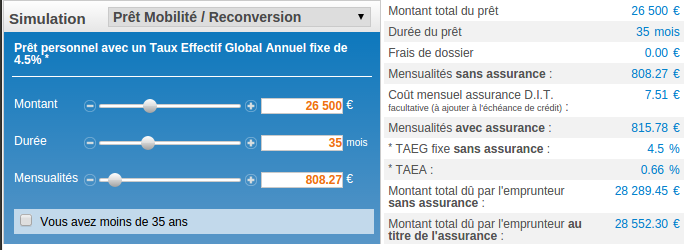
\includegraphics[width=\textwidth]{images/global_simulator1.png} 
	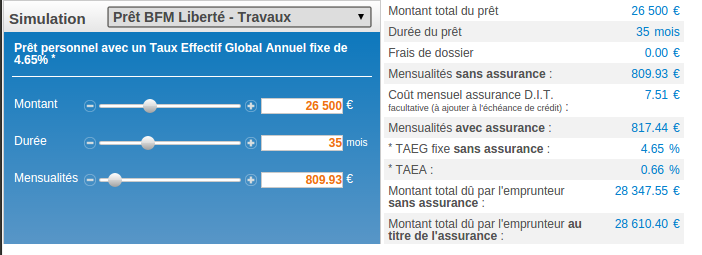
\includegraphics[width=\textwidth]{images/global_simulator2.png} 
	\caption{Simulateur global de prêt}
	\label{global_simulator1}
      \end{figure}
      \paragraph*{Convertir un simulateur d'épargne flash vers une version en HTML5/JavaScript}
      Pour développer ce simulateur j'ai pu reprendre du code existant et l'adapter aux besoins précis de ce cas. Le code est composé en majorité de JavaScript avec le framexork jQuery afin d'afficher le simulateur et de traiter l'intéraction avec l'utilisateur. Une partie de PHP propre à EzPublish est aussi présente afin de récupérer depuis le back-office les données choisis pour les taux d'épargnes. Ceci étant configurable j'ai là aussi créé une classe propre à ce type de simulateur et j'ai ensuite modifié le code pour récupérer les bonnes valeurs. Il n'y a pas eu de difficultés majeurs avec cette fonctionnalité car je me basais sur de l'existant il fallait donc juste faire attention à ne récupérer que le nécessaire et ensuite la partie la plus longue était d'adapter l'affichage pour ressembler à la version originale en flash, ce que j'ai réalisé en CSS (cf. Annexe 1 page \pageref{annexe1}).
      \begin{figure}
	\center
	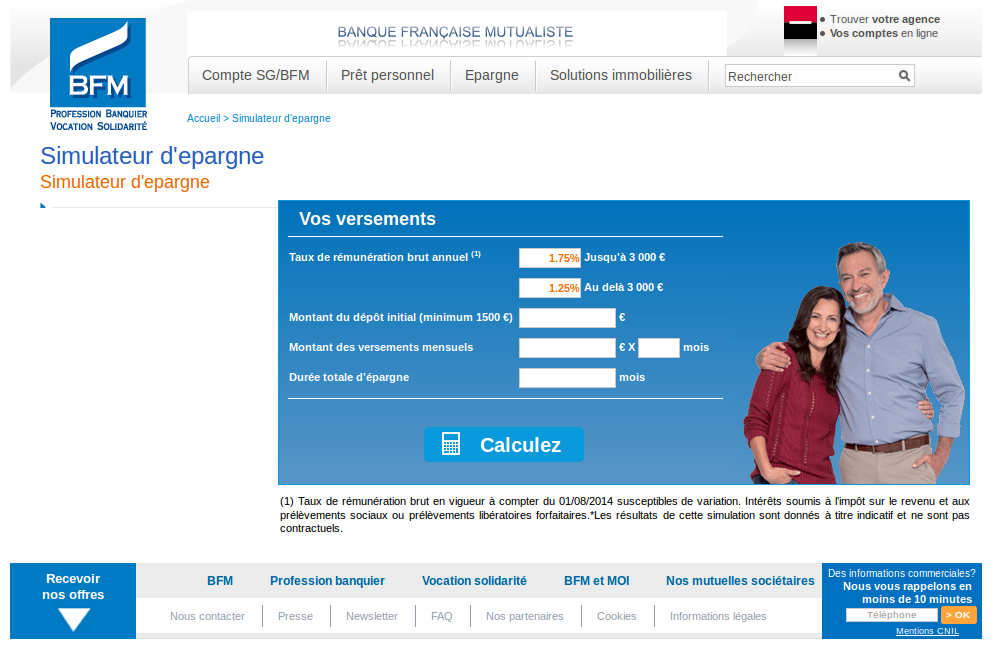
\includegraphics[width=\textwidth]{images/simu_epargne1.png} 
	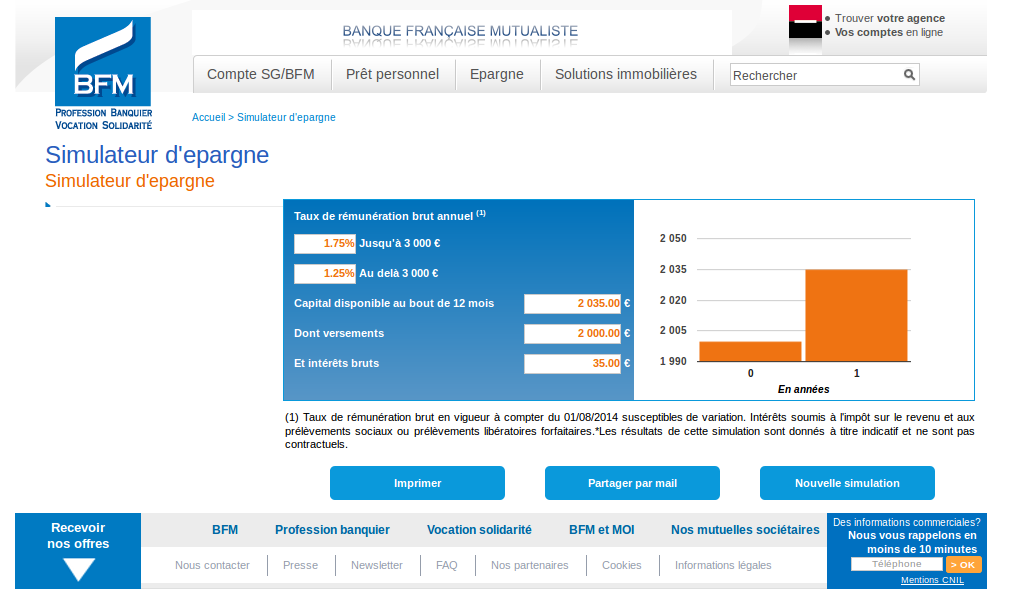
\includegraphics[width=\textwidth]{images/simu_epargne2.png} 
	\caption{Simulateur d'épargne}
	\label{epargne_simulator}
      \end{figure}
      \paragraph*{Développer un template intégré à EzPublish pour la création de landing page et réaliser un exemple en s'inspirant de l'existant}
      Dans le cadre de la création de landing page le client avait l'habitude de développer des pages à part hors du CMS puis de les déposer sur le serveur. Ceci pose problème pour la maintenance et rend la page non contribuable depuis le back-office d'EzPublish. J'ai donc commencé par créé une nouvelle classe dans EzPublish pour les landing page et j'ai ensuite codé un nouveau layout avec uniquement les entêtes de la page et la structure HTML. Le contenu de la page devant être entièrement contribuable depuis le back-office le code était assé simple et consistait juste à récupérer les données. Afin de vérifier le bon fonctionnement j'ai intégrer les landing page existentes directement dans le CMS.
      \begin{figure}
	\center
	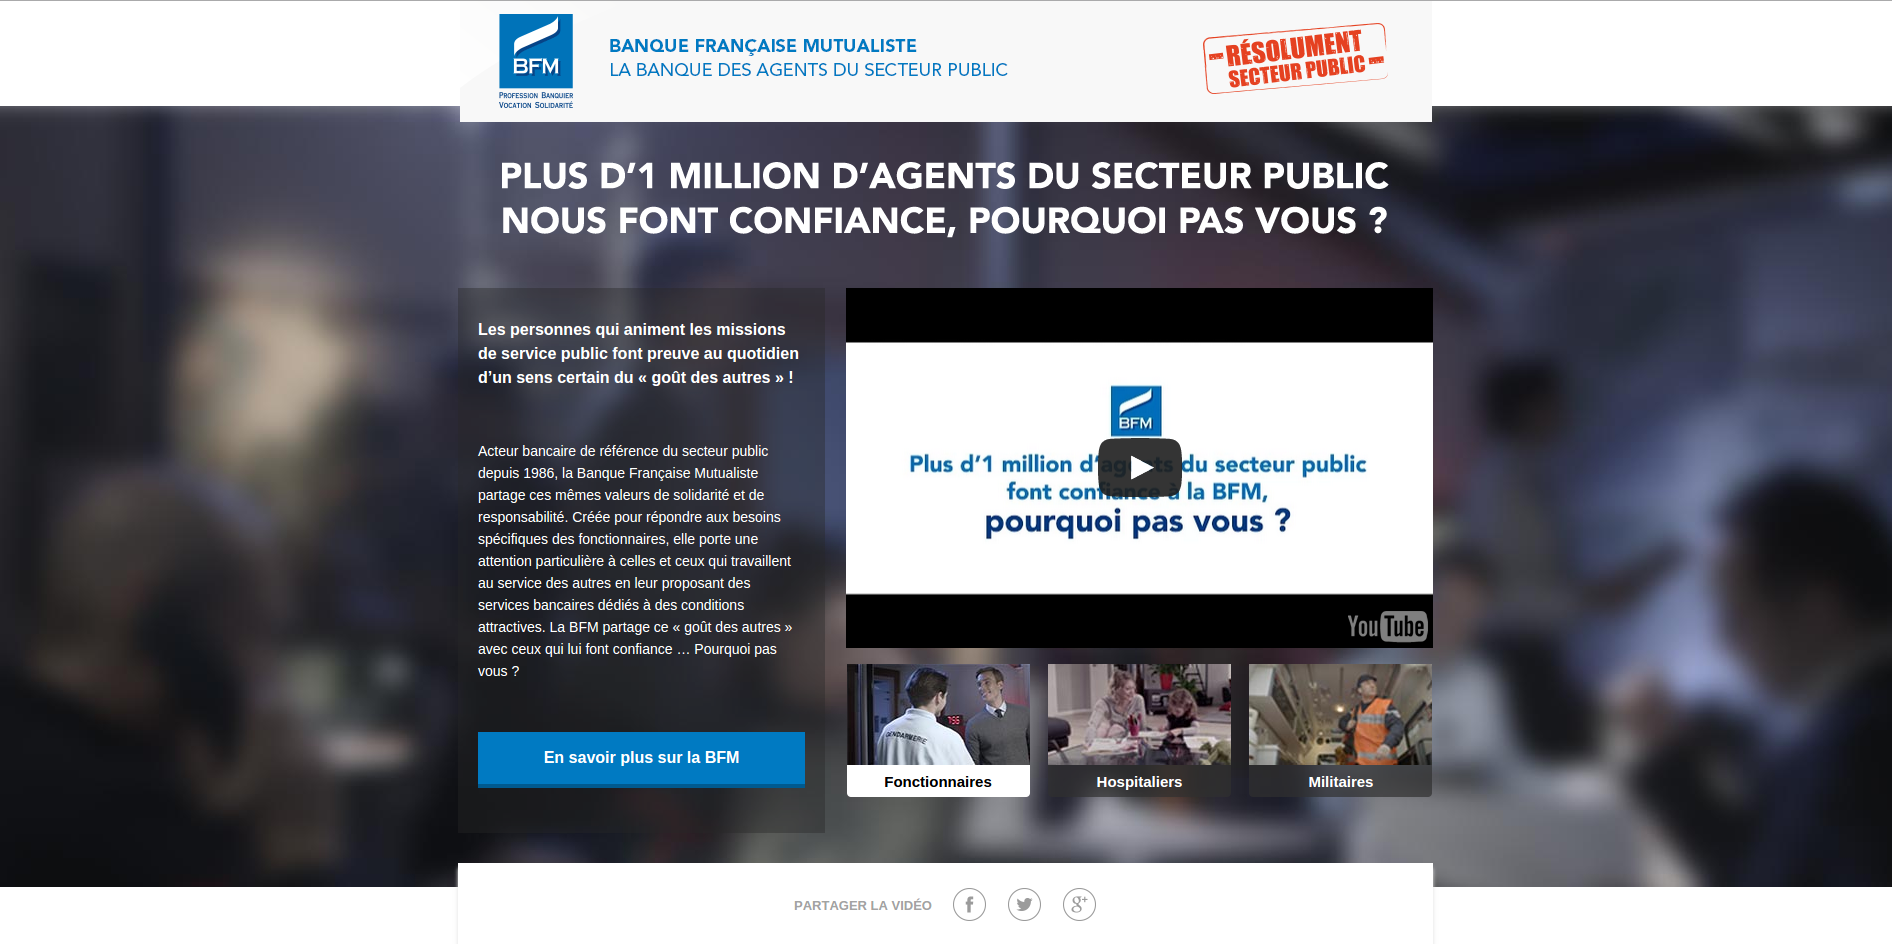
\includegraphics[width=\textwidth]{images/landing_page1.png} 
	\caption{Landing page}
	\label{landing_page}
      \end{figure}
      \paragraph*{Développer un nouvel élément de formulaire permettant la redirection vers une page produit existant et transmettant les données déjà saisies par l'utilisateur}
      Ce développement était un des plus complexes à réaliser car presque tous les éléments devaient être configurables depuis le back-office et les données capables de passer d'un formulaire à l'autre. J'ai donc commencé par créer la classe dans EzPublish avec un bouton radio oui/non afin de lancer la redirection vers un formulaire existant. Ensuite un champ pour sélectionner le formulaire vers lequel pointer et un champ pour le message à afficher lors de la redirection. 
      J'ai ensuite créé le type d'élément à ajouter dans les formulaires que j'ai nommé «Produit Existant». C'est ici que l'essentiel du code s'est écrit, l'idée étant de récupérer les questions du formulaire vers lequel on pointe puis de comparer si les champs existent aussi dans le formulaire actuel. Si tel est le cas alors je transmet les données saisies par l'utilisateur lors de la redirection si celle-ci est actionnée. 
      La première partie de récupération des champs existant sur le formulaire distant se fait grâce aux méthodes fournient par le CMS et on créé ainsi des champs cachés qui permettront la transmission des données. 
      \lstinputlisting[language=php, firstline=1, lastline=24]{question_conditionnelle_1.php}
      Encore une fois la deuxième partie du développement s'est effectuée en JavaScript avec le framework jQuery. Je devais récupérer les donées saisies par l'utilisateur à chaque fois qu'il quittait un champ puis les transmettre dans les champs récupérés cachés du formulaire vers lequel on pointe. Ensuite on vérifie si l'utilisateur choisi l'option «Produit Existant» et si tel est le cas on affiche la popin avec le message indiquant la redirection vers le nouveau formulaire tout en transmettant les données déjà saisies (cf. Annexe 2 page \pageref{annexe2}).
      \paragraph*{Développer une page Web à disposition des téléconseillers intégrant une page d’orientation vers les différentes simulation de prêts personnels et une fonctionnalité d’envoi de mail type intégrant un lien vers une simulation avec des paramètres intégrés dans l’URL}
      Cette page se décompose en deux parties, il en sera donc de même pour le code. Dans un premier temps une section où l'on choisie le prêt que l'on souhaite puis on indique le montant et la durée de celui-ci et enfin on le simule. Ceci génère une URL avec les paramètres intégrés et ouvre une popin avec le simulateur et les valeurs choisies. Le sélecteur de prêt se génère en récupérant les données du back-office qui est configurable en choisissant les prêts à intégrer. Ensuite avec du Javascript on récupère les valeurs saisies par l'utilisateur et on concatène celles-ci à l'URL originale du simulateur pour en former une nouvelle intégrant ces paramètres. 
      \begin{figure}
	\center
	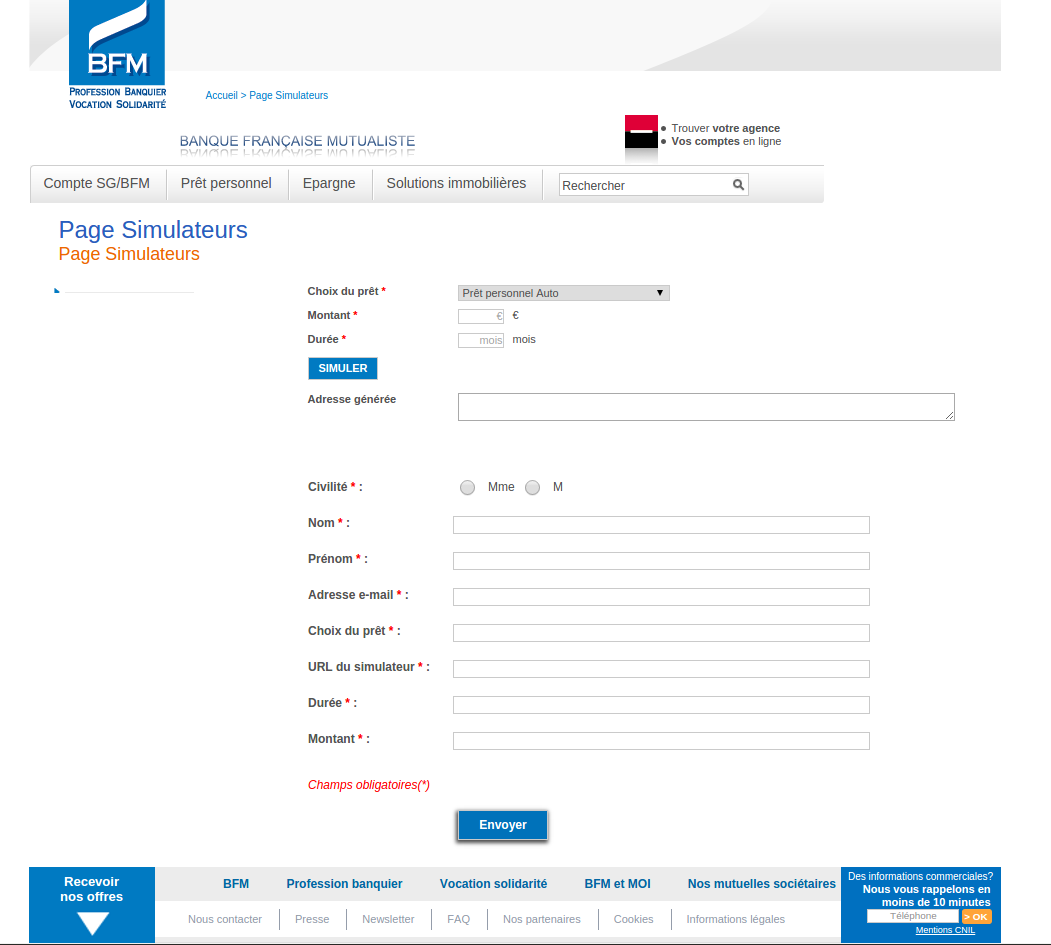
\includegraphics[width=\textwidth]{images/page_teleconseille1.png}  
	\caption{Pages téléconseillers formulaire}
	\label{page_teleconseille_formulaire}
      \end{figure}
      La deuxième section de cette page est un formulaire qui récupère toujours en JavaScript les données saisies pour la simulation plus haut ainsi que l'URL générée et permet de remplir les coordonnées du destinataire et de lui envoyer toutes les informations par mail. Ce mail devant être configurable dans le back-office et offrir la possibilité de récupérer les informations saisies par l'utilisateurs et de les réintégrer dans le mail aussi bien pour l'utilisateur que pour le webmaster. 
      Nous avons rencontré des problèmes de comlptabilité avec IE pour l'ouverture de la popin intégrant le simulateur, en effet le code initial était compatible avec Chrome et Firefox mais pas avec IE9 il a donc fallu le repenser afin de le rendre fonctionnelle sous tous les navigateurs.
      \begin{figure}
	\center
	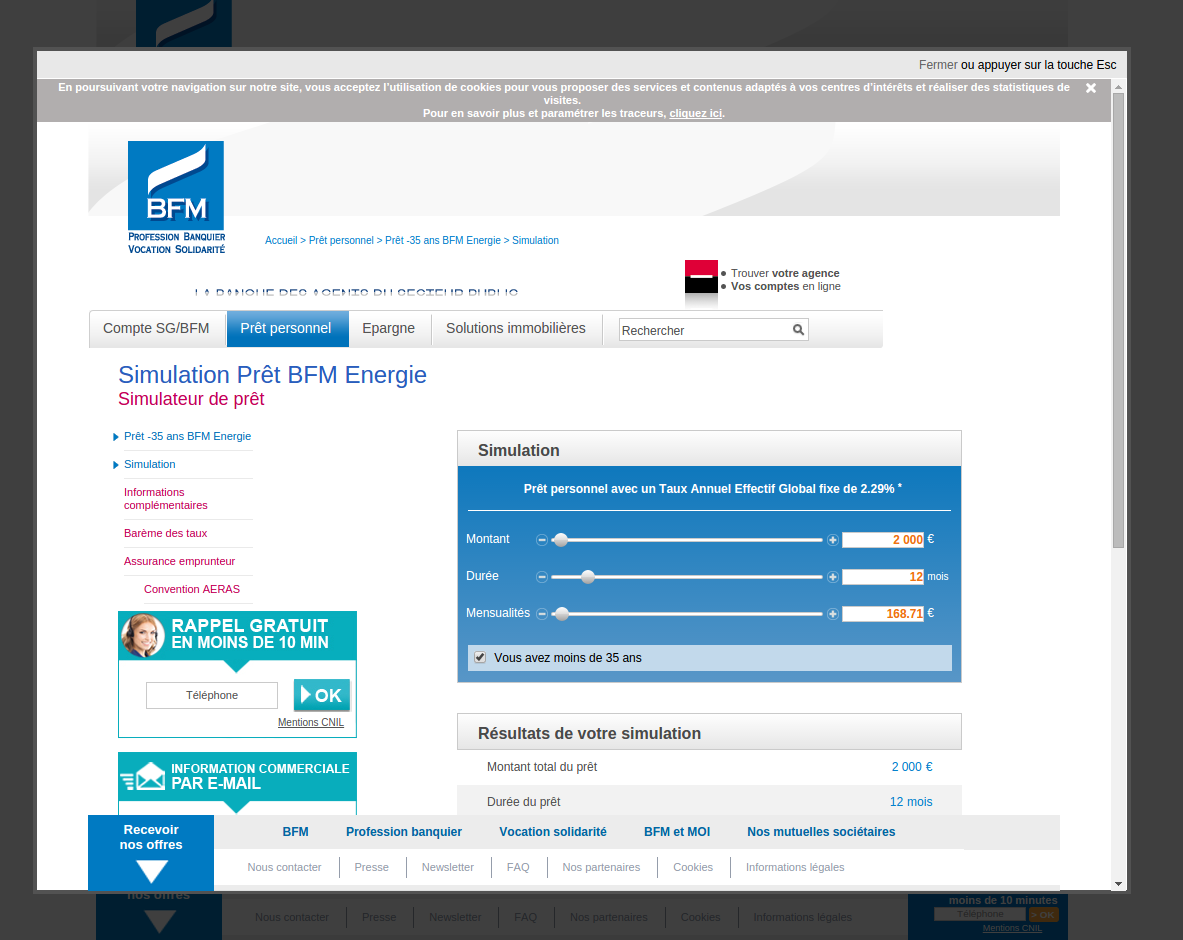
\includegraphics[width=\textwidth]{images/page_teleconseille2.png} 
	\caption{Pages téléconseillers popin simulation}
	\label{page_teleconseille_popin_simulation}
      \end{figure}
      \begin{figure}
	\center
	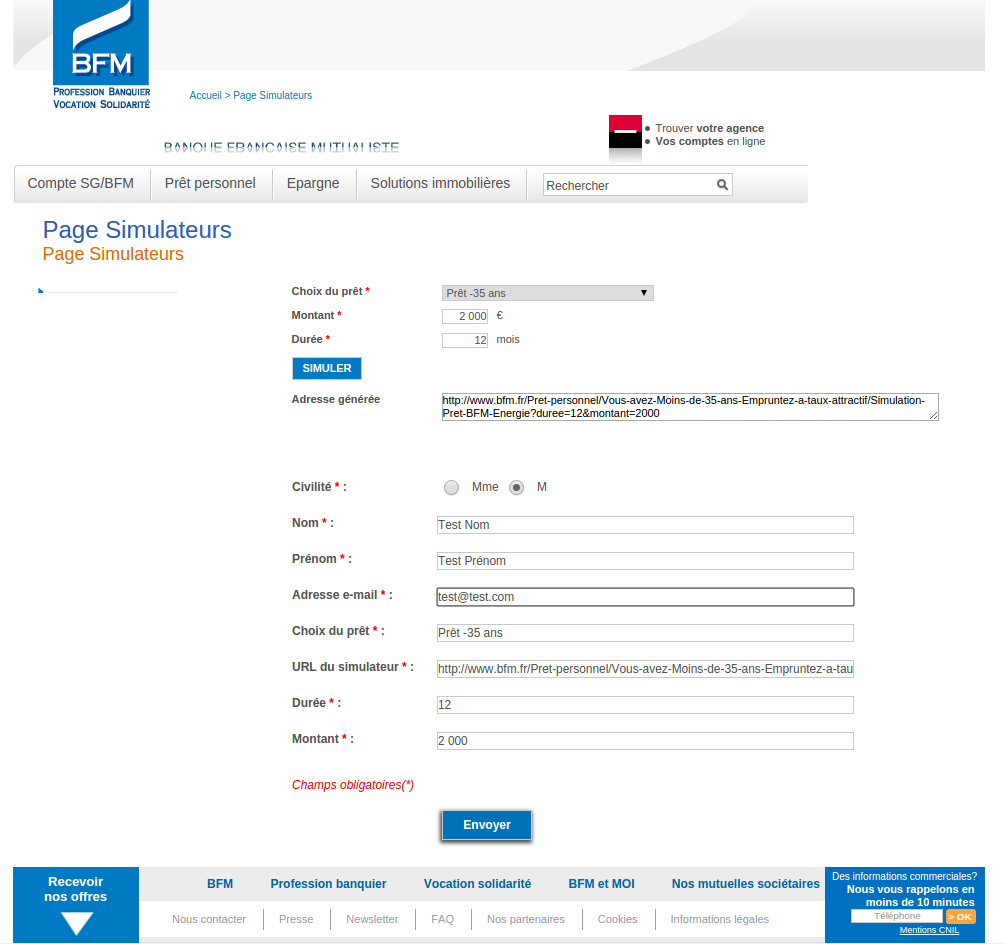
\includegraphics[width=\textwidth]{images/page_teleconseille3.png} 
	\caption{Pages téléconseillers formulaire préremplie}
	\label{page_teleconseille_formulaire_prerempli}
      \end{figure}
    \subsection*{Bilan du projet}
    \addcontentsline{toc}{subsection}{Bilan du projet}%Ajout de l'élément dans le sommaire
    Pour ce second travail avec EzPublish j'ai eu l'occasion d'exercer sur un projet d'envergure et de longue haleine. En effet BFM étant un client de TMA de nombreuses corrections, améliorations ou corrections sont sans cesses à apporter. Ceci offre une vrai diversité dans le projet et le rend donc très intéressant en sois mais aussi pour se former sur la technologie car il permet de couvrir une grande partie des possibilités du CMS. D'un point de vu relationnel ce projet m'a permis d'aborder un nouvel aspect du métier d'ingénieur, à savoir la relation avec le client. J'ai été amené à plusieurs reprises à avoir des rendez-vous téléphoniques afin de discuter de l'avancement des tâches, des modifications à effectuer ou même parfois d'expliquer certains points techniques au client pour qu'il puisse configurer le site à ses souhaits. Pour ce qui est du technique, je suis rentré véritablement dans le coeur du métier avec du PHP, du JavaScript et du style. Autant de langages peut vu en cours mais relativement simple à prendre en main que ce soit en s'inspirant de l'existant ou en recherchant sur internet. Le CMS lui aussi m'était inconnue mais j'ai pu compter sur les autres membres du projet pour m'aider et me conseiller ce qui m'a permis d'appréhender les tâches à effectuer dans de bonnes conditions. J'ai donc beaucoup appris sur ce projet que ce soit sur le plan humain ou technique et même si par la suite je vais être amené à changer de technologie et passer sur du e-commerce avec Magento, il n'en reste pas moins que les langages du WEB sont les mêmes notamment le JavaScript, CSS ou HTML et que PHP est aussi le langage serveur utilisé. Je noterai quand même quelques difficultés rencontrées au cours de ce projet, par exemple les appels au client qui n'étaient pas simple au début par manque d'expérience dans ce domaine. Il est difficile de se mettre à la portée de la personne que nous avons au téléphone et d'être clair, précis et concis quand nous expliquons le problème rencontré ou les actions à effectuer. Enfin la difficulté technique majeure de ce projet et qui à fortiori à engendrer une complication de communication, est que nous n'avions pas accès aux serveurs de productions et de pré-production comme je l'ai expliqué plus tôt. Ceci a rendu difficile les processus de livraison où le client lui même devait effectuer certaines manipulations et nous a obligé à être très précis et patient dans nos explications. Parfois nous avions des bugs que nous n'arrivions pas à reproduire en interne et ne pouvions pas voir ce qu'il se passait dans les logs rendant la tâche de debug compliquée. Bilan positif encore une fois et qui me motive pour le prochain projet qui m'attend avec en plus la découverte d'une nouvelle technologie, Magento.
    
\newpage
    
  \section{POC (Proof Of Concept) thème responsive Gifi}
    \subsection*{Présentation du projet et état de l'art}
    \addcontentsline{toc}{subsection}{Présentation du projet et état de l'art}%Ajout de l'élément dans le sommaire
    L'idée de ce « mini-projet » ou POC était de vérifier la faisabilité d'un changement de thème sans modifier la version de l'application. Le site e-commerce de Gifi étant dans une ancienne version sans thème responsive d'intégré nous voulions récupérer le thème responsive natif de la nouvelle version de Magento et vérifier que sa mise en place ne casse pas le design actuel du site. 
    \subsection*{Mes objectifs}
    \addcontentsline{toc}{subsection}{Mes objectifs}%Ajout de l'élément dans le sommaire
      \begin{itemize}

	\item Intégrer le thème responsive d'un Magento 1.14 sur un Magento 1.13 

      \end{itemize}
    \subsection*{Mes réalisations}
    \addcontentsline{toc}{subsection}{Mes réalisations}%Ajout de l'élément dans le sommaire
    J'ai donc commencé par récupérer la version correspondante à celle mise en place sur le site de Gifi (Magento 1.13), je l'ai installé sur ma LXC afin de pouvoir commencer le test. Ensuite j'ai copié le thème responsive de Magento 1.14 et je l'ai chargé depuis le back-office. Il s'agissait ensuite d'effectuer des tests de compatibilité pour voir si des modules natifs de Magento ne fonctionnait plus. Les fiches produits notamment ne s'affichait plus correctement car une fonction n'était plus déclaré au même endroit dans le code. J'ai donc remonté ces petits beugs et confirmé la faisabilité de ce « backportage » de thème. 
    \subsection*{Bilan du projet}
    \addcontentsline{toc}{subsection}{Bilan du projet}%Ajout de l'élément dans le sommaire
    Plus qu'un projet en tant que tel j'ai découvert par le biais de cette mission une autre facette du métier. En effet il n'est pas rare que les clients demandent pour ce genre d'expertise afin de savoir approximativement la faisabilité d'une évolution et surtout son coût. Car le POC a aussi pour vocation de donner un ordre d'idée du temps nécessaire à la réalisation et donc le budget à y consacrer. C'est donc un bon moyen pour le client de se rendre compte si l'investissement en vaut la peine ou s'il est préférable de se passer de ce développement et de consacrer le budget à autre chose. D'un point de vu purement technique cela m'a permis de prendre en main Magento et de bien assimiler les notions de thème, de layout et de template qui sont des aspects clés des projets où je serai amené à travailler par la suite. 

    \newpage
    
  \section{Refonte graphique Darjeeling}
    \subsection*{Présentation du projet et état de l'art}
    \addcontentsline{toc}{subsection}{Présentation du projet et état de l'art}%Ajout de l'élément dans le sommaire
    Darjeeling fait partie des clients de Smile depuis relativement longtemps, le site initial a été réalisé par le groupe. Il s'agit d'un site e-commerce de lingerie proposant de nombreux produits et les services associés, il est à noter que des magasins physiques sont présents partout en France. Aujourd'hui nous intervenons dans le cadre d'une refonte graphique et allons modifier principalement les templates, les styles et s'assurer de ne pas dégrader le résultat sur mobile. Il n'y a donc pas ou très peu de développement fonctionnel sur ce projet, uniquement du visuel. Les technologies utilisées n'en sont pas moins intéressantes, notamment le système mis en place pour la compilation des fichiers de style et JavaScript. En effet nous utilisons Sass (Syntactically Awesome Style Sheets) qui est une sorte d'amélioration du language CSS et qui y ajoute certaines fonctionnalités. Ces fichiers doivent être ensuite compilé pour obtenir un CSS qui est le seul langage compris par les navigateurs. Pour ce faire nous utilisons Grunt qui surveille toutes modifications apportées aux fichiers Sass et qui nous seulement les compile mais les minifie aussi. Au final nous obtenons un seul et unique gros fichier CSS qui est la concaténation de tous les fichiers Sass. Ceci permet de développer sur des fichiers séparés et clairs puis de livrer au serveur un fichier unique ce qui est préférable en terme de performance. Comme la plupart des projets la principale difficulté sera le temps, car nous avons eu un peu plus de 2 mois pour réaliser le projet.
    \subsection*{Mes objectifs}
    \addcontentsline{toc}{subsection}{Mes objectifs}%Ajout de l'élément dans le sommaire
      \begin{itemize}

	\item Refonte du template et du style de divers pages du site
	\item Refonte de la liste produits et de ses filtres
	\item Optimisation du nouveau design sur mobile
	\item Phase de recette avec le client

      \end{itemize}
    \subsection*{Mes réalisations}
    \addcontentsline{toc}{subsection}{Mes réalisations}%Ajout de l'élément dans le sommaire
    	\paragraph*{Refonte du template et du style de divers pages du site}
	Il s'agit pour moi de mon premier gros projet en utilisant Magento, j'ai donc commencé par réaliser la refonte des pages les plus simples à savoir le header et le footer. J'ai donc redesigné ces pages en suivant les maquettes graphiques fournient pas le client. Il y avait notamment des changements de logos, d'icônes, de couleurs et de polices mais aussi quelques modifications fonctionnelles comme le changement des liens présents dans le header et le menu de navigation. J'ai eu par exemple à ajouter des champs de le back-office permettant au contributeur d'ajouter une image et lien de promotion directement dans le menu. Ceci doit être configurable, j'ai donc commencé par développer un « installer » qui permet l'ajout d'attributs dans le back-office (par modification de la base de données), un pour le choix d'une image et l'autre pour le lien vers lequel pointe cette image (cf. Annexe 3 page \pageref{annexe3}). J'ai ensuite modifié le template du menu afin de faire appel à ces attributs et ainsi afficher le contenu ajouté. Finalement j'ai adapté le style pour respecter la mise en forme souhaitée par le client. Pour le footer la partie mise en forme était assez simple, du style CSS sans complexité, la fonctionnalité intéressante réside dans la récupération des liens que l'on affiche dans celui-ci. Un attribut position avait été ajouté et je l'ai donc utilisé afin d'offrir la possibilité au contributeur de choisir dans quelle partie du footer il souhaitait positionner le lien. Il ne me restait plus qu'à mettre en place une boucle dans le template qui parcoure les éléments et récupère leur lien pour les afficher.
	\lstinputlisting[language=html, firstline=1, lastline=19]{footer_recuperation_darjeeling.html}
	Par la suite j'ai réalisé la page « Mes envies » qui regroupe les produits sélectionnés par l'utilisateur et lui permet soit de les ajouter à son panier soit de les retirer de cette liste. J'ai donc redesigné la page ainsi que les blocs qui affiche les produits et implémenté un script pour l'affichage d'info bulle custom. Il s'agit uniquement de développement front, du templating et du style mais aussi du JavaScript. Sachant que cette info bulle devrait être présente à plusieurs endroits dans le site j'ai mis en place un petit script jQuery permettant de vérifier si le produit est déjà dans la liste « Mes envies » au quel cas on propose d'enlever le produit. Dans le cas contraire l'info bulle affiche « Ajouter à mes envies ». Ce scipt doit être capable de réagir au clique sur le bouton et au chargement de la page, j'utilise pour ça les observateurs jQuery (cf. Annexe 4 page \pageref{annexe4}).
	\paragraph*{Refonte de la liste produits et de ses filtres}
	La liste produits est un template appelé à différents endroits du site notamment lorsque l'on sélectionne une catégorie particulière ou que l'on effectue une recherche. Ce template est chargé de lister les produits comme son nom l'indique, de mettre en place une pagination et de proposer divers filtres pour trier les résultats. Pour ce qui est de l'affichage j'ai mis en place un nouveau design de blocs sur 3 colonnes respectant les maquettes. Le client souhaitait afficher 48 produits par pages et proposer un lien en bas permettant de charger les 48 produits suivants. J'ai donc implémenté cette fonctionnalité par le biais d'un appel AJAX qui charge les éléments sans avoir à recharger toute la page. J'ai aussi adapté le template pour répondre à ces nouveaux besoins. Les blocs affichant les produits ont aussi été modifié en ajoutant de nouvelles fonctionnalités d'achat et de déplacement dans la liste de souhait. J'ai notamment utilisé le script développé et cité précédemment. Concernant la partie filtre j'ai repris le fonctionnement qui était déjà en place en terme de fonctionnalités et j'ai ajouté des éléments de design en plus de la refonte graphique. Ceci s'est traduis par l'utilisation de JavaScript pour mettre en place une liste déroulante permettant d'afficher ou non le détail des filtres. Ainsi qu'un scipt qui regarde qu'elles filtres sont actifs au changement ou rechargement de la page et les réouvre directement dans le but améliorer l'expérience utilisateur. 
	\lstinputlisting[language=html, firstline=1, lastline=31]{script_accordion_active.html}
	\paragraph*{Optimisation du nouveau design sur mobile}
	Le site mobile de Darjeeling venait tout juste d'être refait par Smile, il s'agissait donc juste d'impacter les principaux changements graphiques sur cette plateforme. Uniquement du développement graphique, changement de couleurs, de logos,... Enfin j'ai dû m'assurer que les changements fonctionnels sur le site desktop ne cassait pas le fonctionnement sur mobile puisque certains modules sont repris dans les deux cas. 
	\paragraph*{Phase de recette avec le client}
	Une fois les développements terminés nous avons passé le projet sur le serveur de préproduction afin que le client puisse regarder et tester ce qui avait été fait. L'intérêt de cette phase est d'avoir les retours du client et si une anomalie est détectée il créé un ticket sur Redmine (notre plateforme de gestion de projet) nous indiquant le problème rencontré. Celui-ci est ensuite vérifié par le chef de projet par s'assurer qu'il s'agit bien d'une anomalie rentrant dans le périmètre du projet et non une évolution à facturer en plus au client. Dans le premier cas le ticket est affecté à un développeur qui va corriger le problème puis le relivrer pour que le client puisse s'assurer que tout est réglé. L'intérêt pour moi durant cette phase du projet a été de pouvoir évoluer sur l'ensemble du site et non uniquement sur le développement que j'avais effectué lors de la phase précédente. En effet j'ai été amené à corriger des bugs, apporter des modifications ou même ajouter de nouvelles fonctionnalités sur des pages qui ne me concernaient pas initialement. Par exemple l'ajout d'un lien configurable sur un widget de la home page. Je n'avais pas travaillé avec les widget tout au long du projet et là ça a été l'occasion pour moi de les découvrir. J'ai donc ajouté un attribut au widget permettant au contributeur de sélectionner si oui ou non il souhaite que le lien s'affiche. Puis dans le template ajouter une condition sur l'affichage du lien en récupérant l'information saisie dans le BO.  
    \subsection*{Bilan du projet}
    \addcontentsline{toc}{subsection}{Bilan du projet}%Ajout de l'élément dans le sommaire
    Lorem ipsum dolor sit amet, consectetur adipiscing elit. Nullam pharetra sem neque, at lacinia tellus rhoncus sed. Aliquam erat volutpat. Sed in facilisis dolor. Nam gravida purus vel ante auctor, non venenatis mauris scelerisque. Maecenas odio nunc, dapibus eu varius ac, dapibus non diam. Nam a ligula sit amet velit porta auctor. Vestibulum vel luctus eros. Sed vestibulum neque tristique, fringilla felis sed, pharetra dui. Nulla facilisi. Aliquam viverra velit nulla, ut placerat purus auctor vitae. Aenean vitae mauris tristique metus placerat ultrices vel ac magna. Vestibulum massa leo, faucibus nec tincidunt vitae, bibendum vel tortor. Aliquam erat volutpat.
    
        \newpage
    
  \section{Snowleader refonte 2015}
    \subsection*{Présentation du projet et état de l'art}
    \addcontentsline{toc}{subsection}{Présentation du projet et état de l'art}%Ajout de l'élément dans le sommaire
    Snowleader, c'est la référence en e-commerce pour le snow, la glisse et l'outdoor avec un catalogue de plus de 15000 références. Pour Smile Sud-Ouest cela est synonyme d'un gros projet avec de nombreuses demandes et aussi bien sur le design que sur les fonctionnalités. Comme sur les autres projets nous avons des contraintes de temps bien entendu mais aussi de performance car le catalogue est vaste ce qui fait beaucoup de données à traiter et enfin de compatibilité, en effet le design original doit s'afficher correctement sur tous les navigateurs et être responsive sur tablette (nous ne nous occupons pas du mobile car un site à part y est dédié). Qui dit projet conséquent, dit de nombreuses attentes de la part du client, de la précision en terme de rendu et donc une charge de travail élevée pour l'agence. C'est donc avec un équipe projet conséquente que le projet a été mené soit une dizaine de personnes, ce qui représente presque un quart des collaborateurs de Smile Sud-Ouest. Pour ma part je n'ai pas rejoins le projet dès son commencement car je travaillais sur autre chose, je suis venu en renfort au vu des besoins de développement. En effet la majorité des pages du site sont à refaire aussi bien en terme de design que d'agencement ou de fonctionnalité. Nous avons à notre disposition bon nombre de maquettes graphiques ainsi que des spécifications techniques détaillées pour nous aider dans notre travail. Ma tâche principale est l'espace client, ce qui regroupe les pages de connexions et de déconnexions, le dashboard avec l'accès à toutes les données clients (historique de commandes, points de fidélités, ...) et les divers formulaires d'inscriptions ou de modification d'informations. 
    \subsection*{Mes objectifs}
    \addcontentsline{toc}{subsection}{Mes objectifs}%Ajout de l'élément dans le sommaire
      \begin{itemize}

	\item Donec vitae erat enim. Maecenas tempus egestas sem, sit amet condimentum justo consectetur sed. Donec quis iaculis 
	\item urna. Donec sodales lobortis diam, at consequat erat bibendum pulvinar. Nunc eu ultricies justo, eget viverra ligula. 
	\item Pellentesque quis tincidunt elit, eu ultrices nisi. Praesent consectetur semper cursus. In hac habitasse platea dictumst. 

      \end{itemize}
    \subsection*{Mes réalisations}
    \addcontentsline{toc}{subsection}{Mes réalisations}%Ajout de l'élément dans le sommaire
    Lorem ipsum dolor sit amet, consectetur adipiscing elit. Nullam pharetra sem neque, at lacinia tellus rhoncus sed. Aliquam erat volutpat. Sed in facilisis dolor. Nam gravida purus vel ante auctor, non venenatis mauris scelerisque. Maecenas odio nunc, dapibus eu varius ac, dapibus non diam. Nam a ligula sit amet velit porta auctor. Vestibulum vel luctus eros. Sed vestibulum neque tristique, fringilla felis sed, pharetra dui. Nulla facilisi. Aliquam viverra velit nulla, ut placerat purus auctor vitae. Aenean vitae mauris tristique metus placerat ultrices vel ac magna. Vestibulum massa leo, faucibus nec tincidunt vitae, bibendum vel tortor. Aliquam erat volutpat.
    \subsection*{Bilan du projet}
    \addcontentsline{toc}{subsection}{Bilan du projet}%Ajout de l'élément dans le sommaire
    Lorem ipsum dolor sit amet, consectetur adipiscing elit. Nullam pharetra sem neque, at lacinia tellus rhoncus sed. Aliquam erat volutpat. Sed in facilisis dolor. Nam gravida purus vel ante auctor, non venenatis mauris scelerisque. Maecenas odio nunc, dapibus eu varius ac, dapibus non diam. Nam a ligula sit amet velit porta auctor. Vestibulum vel luctus eros. Sed vestibulum neque tristique, fringilla felis sed, pharetra dui. Nulla facilisi. Aliquam viverra velit nulla, ut placerat purus auctor vitae. Aenean vitae mauris tristique metus placerat ultrices vel ac magna. Vestibulum massa leo, faucibus nec tincidunt vitae, bibendum vel tortor. Aliquam erat volutpat.


% Faire une bande chronologique en expliquant ce que je faisais dans le temps type frise chronologique    
    
    
\chapter*{Conclusion}
\addcontentsline{toc}{chapter}{Conclusion}%Ajout de l'élément dans le sommaire
  \section*{Enseignements et bénéfices}
  \addcontentsline{toc}{section}{Enseignements et bénéfices}%Ajout de l'élément dans le sommaire
  \section*{Les projets à venir}
  \addcontentsline{toc}{section}{Les projets à venir}%Ajout de l'élément dans le sommaire

\chapter*{Annexes}
\thispagestyle{\chead{}}
\addcontentsline{toc}{chapter}{Annexes}%Ajout de l'élément dans le sommaire
  \section*{Annexe 1}
  \addcontentsline{toc}{section}{Annexe 1}%Ajout de l'élément dans le sommaire
  \label{annexe1}
  \lstinputlisting[language=HTML, firstline=1, lastline=68]{saving_simulator_html5.html}
  \section*{Annexe 2}
  \addcontentsline{toc}{section}{Annexe 2}%Ajout de l'élément dans le sommaire
  \label{annexe2}
  \lstinputlisting[language=HTML, firstline=1, lastline=63]{question_conditionnelle_2.html}
  \section*{Annexe 3}
  \addcontentsline{toc}{section}{Annexe 3}%Ajout de l'élément dans le sommaire
  \label{annexe3}
  \lstinputlisting[language=php, firstline=1, lastline=51]{installer_darjeeling.php}
  \section*{Annexe 4}
  \addcontentsline{toc}{section}{Annexe 4}%Ajout de l'élément dans le sommaire
  \label{annexe4}
  \lstinputlisting[language=html, firstline=1, lastline=31]{script_tooltip.html}
%Table des illustrations
\listoffigures
\thispagestyle{\chead{}}

\end{document}